\documentclass[14pt,a4paper, oneside]{extreport}

\usepackage{etex} % расширение классического tex
% в частности позволяет подгружать гораздо больше пакетов, чем мы и займёмся далее
\usepackage{etoolbox} % логические операторы для своих макросов

 % Нужен уже здесь для корректной работы шрифтов в хетехе

%%%%%%%%%% Математика %%%%%%%%%%
\usepackage{amsmath,amsfonts,amssymb,amsthm,mathtools} 
% Показывать номера только у тех формул, на которые есть \eqref{} в тексте.
%\mathtoolsset{showonlyrefs=true} 
%\usepackage{leqno} % Нумерация формул слева


%%%%%%%%%%%%%%%%%%%%%%%%%%%%%%%%%%%%%%%%%%%%%%%%%%%%%%%%%%%%%%%%%
%%%%%%%%%%%%%%%%%%%%%%%% Шрифты %%%%%%%%%%%%%%%%%%%%%%%%%%%%%%%%%
%%%%%%%%%%%%%%%%%%%%%%%%%%%%%%%%%%%%%%%%%%%%%%%%%%%%%%%%%%%%%%%%%

% Если не нужен какой-то конкретный шрифт и устраивает computer modern по умолчанию или есле по какой-то причине не работает хелатех, то активаруем первый кусок.
% \usepackage[T2A]{fontenc}             % поддержка кириллицы в LaТеХ
% \usepackage[utf8]{inputenc}           % по умолчанию кодировка Windows
% \usepackage[english,russian]{babel}   % определение языков в документе

%------------------------------------------------------------------
% XeTeX прибамбасы. Для активации этих бравых ребят необходимо установить полный miktex! (не on the fly), прописать в настройках техмaker в графе latex : xelatex -interaction=nonstopmode %.tex

% После надо поставить вместо быстрой сборки XeLaTeX или LuaLaTeX и скорее всего ничего работать не будет. Придётся гуглить и танцевать с бубном. В случае LuaLaTeX у меня шла сборка pdf файла, но при этом выдавалась странная ошибка.

%XeLaTeX позволяет очень гибко работать со шрифтами.

\usepackage{fontspec}

\defaultfontfeatures{Mapping=tex-text}

\setmainfont{Linux Libertine O} % or Helvetica, Arial, Cambria
% why do we need \newfontfamily:
% http://tex.stackexchange.com/questions/91507/
\newfontfamily{\cyrillicfonttt}{Linux Libertine O}
\newfontfamily{\cyrillicfont}{Linux Libertine O}
\newfontfamily{\cyrillicfontsf}{Linux Libertine O}


\usepackage{unicode-math}
\setmathfont[math-style=ISO]{Asana Math}       % шрифт для математики

\usepackage{polyglossia}
\setdefaultlanguage{russian}
\setotherlanguage{english}

%%%%%%%%%%%%%%%%%%%%%%%%%%%%%%%%%%%%%%%%%%%%%%%%%%%%%%%%%%%%%%%%%

%%%%%%%%%% Работа с картинками %%%%%%%%%
\usepackage{graphicx}                  % Для вставки рисунков
\usepackage{graphics} 
\graphicspath{{images/}{pictures/}}    % можно указать папки с картинками
\usepackage{wrapfig}                   % Обтекание рисунков и таблиц текстом
\usepackage{subfigure}                 % для создания нескольких рисунков внутри одного


%%%%%%%%%% Работа с таблицами %%%%%%%%%%
\usepackage{tabularx}            % новые типы колонок
\usepackage{tabulary}            % и ещё новые типы колонок
\usepackage{array,delarray}      % Дополнительная работа с таблицами
\usepackage{longtable}           % Длинные таблицы
\usepackage{multirow}            % Слияние строк в таблице
\usepackage{float}               % возможность позиционировать объекты в нужном месте 

%  вычисляемые колонки по tabularx
\newcolumntype{C}{>{\centering\arraybackslash}X}
\newcolumntype{L}{>{\raggedright\arraybackslash}X} 
\newcolumntype{Y}{>{\arraybackslash}X}
\newcolumntype{Z}{>{\centering\arraybackslash}X}


%%%%%%%%%% Графика и рисование %%%%%%%%%%
\usepackage{tikz, pgfplots}      % язык для рисования графики из latex'a
\usepackage{pgfplotstable}
\usetikzlibrary{trees}           % tikz-прибамбас для рисовки деревьев
\usepackage{tikz-qtree}          % альтернативный tikz-прибамбас для рисовки деревьев
\usetikzlibrary{arrows}          % tikz-прибамбас для рисовки стрелочек подлиннее

\usepackage{amscd}                   % Пакеты для рисования 
\usepackage[matrix,arrow,curve]{xy}  % комунитативных диаграмм


%%%%%%%%%% Гиперссылки %%%%%%%%%%
\usepackage{xcolor}              % разные цвета
\usepackage{color}               % и ещё цвета
\usepackage{colortbl}            % совсем много цветов

\usepackage{hyperref}
\hypersetup{				
    unicode=true,           % позволяет использовать юникодные символы
    colorlinks=true,       	% true - цветные ссылки, false - ссылки в рамках
    urlcolor =blue,         % цвет ссылки на url
    linkcolor=black,        % внутренние ссылки
    citecolor=black,        % на библиографию
}
% hyperindex -
% breaklinks -


%%%%%%%%%% Програмный код %%%%%%%%%%
\usepackage{minted}
% Включает подцветку комманд в программах!
% Нужно, чтобы на компе стоял питон, надо поставить пакет Pygments, в котором он сделан через pip или cmd ( нужно ввести easy_install Pygments ). 
% После нужно зайти в настройки texmaker и там прописать в PdfLatex pdflatex -shell-escape -synctex=1 -interaction=nonstopmode %.tex
% Документация по пакету хорошая, сам читал, погуглите!

%%% Если не получилось подключить пакет minted, то для кода можно использовать окружение listing или verbantim, но в этом случае не будет никакого цветного синтаксиса.


%%%%%%%%%% Другие приятные пакеты %%%%%%%%%
\usepackage{multicol}       % несколько колонок
\usepackage{verbatim}       % для многострочных комментариев
\usepackage{makeidx}        % для создания предметных указателей

\usepackage{enumitem} % дополнительные плюшки для списков
%  например \begin{enumerate}[resume] позволяет продолжить нумерацию в новом списке

\usepackage{todonotes} % для вставки в документ заметок о том, что  осталось сделать
% \todo{Здесь надо коэффициенты исправить}
% \missingfigure{Здесь будет Последний день Помпеи}
% \listoftodos --- печатает все поставленные \todo'шки



%%%%%%%%%%%%%%%%%%%%%%%%%%%%%%%%%%%%%%%%%%%%%%%%%%%%%%%%%%%%%%%%%%%
%%%%%%%%%%%%%%%%%%%%% ГОСТОВСКИЕ ПРИБАМБАСЫ %%%%%%%%%%%%%%%%%%%%%%%
%%%%%%%%%%%%%%%%%%%%%%%%%%%%%%%%%%%%%%%%%%%%%%%%%%%%%%%%%%%%%%%%%%%

%%% Параметры страницы
\usepackage{indentfirst} % установка отступа в первом абзаце главы!!!
\usepackage{setspace}
\setlength{\parindent}{1.5em} % Красная строка.
\setstretch{1.33}  % Межстрочный интервал
\usepackage{extsizes} % Возможность сделать 14-й шрифт

%%% размер листа бумаги
\usepackage[paper=a4paper,top=15mm, bottom=15mm,left=35mm,right=10mm,includefoot]{geometry}

\flushbottom       % Эта команда заставляет LaTeX чуть растягивать строки, чтобы получить идеально прямоугольную страницу
\righthyphenmin=2  % Разрешение переноса двух и более символов
\widowpenalty=300  % Небольшое наказание за вдовствующую строку (одна строка абзаца на этой странице, остальное --- на следующей)
\clubpenalty=3000  % Приличное наказание за сиротствующую строку (омерзительно висящая одинокая строка в начале страницы)
\tolerance=1000     % Ещё какое-то наказание.


%%% Нумерация страниц сверху поцентру!
\usepackage{fancyhdr}
\pagestyle{fancy}
\fancyhf{}
\fancyhead[C]{\thepage}
\fancyheadoffset{0mm}  %движение номера вправо
\fancyfootoffset{0mm}
\setlength{\headheight}{10mm}  \renewcommand{\headrulewidth}{0pt} \renewcommand{\footrulewidth}{0pt} %движение вниз
\fancypagestyle{plain}{\fancyhf{} \chead{\thepage}}
%строка выше отвечает за нумерацию страниц с заголовками. Если указать \rhead то нумерация будет идти сверху справа. Если стереть строку, то снизу по центру. 
\setcounter{page}{1} % начать нумерацию страниц с 1


%%% Заголовки
\usepackage{titlesec}{\raggedleft}    % Заголовки по левому краю    

% Редактирования Глав и названий
\titleformat{\chapter} 
    {\normalfont\bfseries\large}
    {\chaptertitlename~\thechapter.}{0.5em}{\normalfont}

% Более низкие уровни
\titleformat{\section}{\bfseries}{\thesection}{0.5em}{}
\titleformat{\subsection}{\bfseries}{\thesubsection}{0.5em}{}

% Убирает чеканутые отступы вверху страницы
\titlespacing{\chapter}{0pt}{-20pt}{15 pt} 
 

% Этот пакет позволяет сделать многие вещи с заголовками и колонтитулами, но более просто и элеганно.
% http://ctan.org/pkg/titletoc

\usepackage{titletoc}								

\titlecontents{chapter}
              [1em] % 
              {\normalsize}
              {\contentslabel{1 em}}
              {\hspace{-1 em}}
              {\normalsize\titlerule*[10pt]{.}\contentspage}

\titlecontents{section}
              [3 em] % 
              {\normalsize}
              {\contentslabel{1.75 em}}
              {\hspace{-1.75 em}}
              {\normalsize\titlerule*[10pt]{.}\contentspage}

\titlecontents{subsection}
              [6 em] % 
              {\normalsize}
              {\contentslabel{3 em}}
              {\hspace{-3 em}}
              {\normalsize\titlerule*[10pt]{.}\contentspage}


% верста содержания по ГОСТ
\usepackage{tocloft}     
\renewcommand{\cftchapaftersnum}{ }
%\renewcommand\cftchappresnum{\space}
\renewcommand{\cftchapnumwidth}{1 em}
\renewcommand{\cftsecaftersnum}{ }
\renewcommand{\cftsecnumwidth}{2.0 em}
\renewcommand{\cftsubsecaftersnum}{ }
\renewcommand{\cftsubsecnumwidth}{3.0 em}
    

% Правильные подписи под таблицей и рисунком 
\usepackage[tableposition=top, singlelinecheck=false]{caption}
\usepackage{subcaption}
	
   \DeclareCaptionStyle{base}% 
		[justification=centering,indention=0pt]{}
   \DeclareCaptionLabelFormat{gostfigure}{Рисунок #2}
   \DeclareCaptionLabelFormat{gosttable}{Таблица #2}
  	
   \DeclareCaptionLabelSeparator{gost}{~---~}   
   \captionsetup{labelsep=gost} 
   
   \DeclareCaptionStyle{fig01}%
           [margin=5mm,justification=centering]%
           {margin={3em,3em}}
   \captionsetup*[figure]{style=fig01,labelsep=gost,labelformat=gostfigure,format=hang}

   \DeclareCaptionStyle{tab01}%
           [margin=5mm,justification=centering]%
           {margin={3em,3em}}
   \captionsetup*[table]{style=tab01,labelsep=gost,labelformat=gosttable,format=hang}

%   межстрочный отступ в таблице
 \renewcommand{\arraystretch}{1.1}

% многостраничные таблицы под РОССИЙСКИЙ СТАНДАРТ
\usepackage{fr-longtable} 

\makeatletter
 \LTcapwidth=\textwidth
\def\LT@makecaption#1#2#3{%
 \LT@mcol\LT@cols c{\hbox to\z@{\hss\parbox[t]\LTcapwidth{%
\sbox\@tempboxa{ #1{#2: } #3}%
 \ifdim\wd\@tempboxa>\hsize
	\hbox to\hsize{\hfil #1#2\mbox{ }}
     	\hbox to\hsize{\hfil \parbox[c]{0.9\textwidth}{\centering #3}\hfil }%%
 \else
     \hbox to\hsize{\hfil #1#2\mbox{ }}
     \hbox to\hsize{\hfil #3\hfil}%
 \fi
 \endgraf\vskip 0.5\baselineskip}%
 \hss}}}
\makeatother


%Более гибкие спсики
\usepackage{enumitem}
\makeatletter
\AddEnumerateCounter{\asbuk}{\russian@alph}{щ}
\makeatother


%%% ГОСТОВСКИЕ СПИСКИ!!!
% ГОСТ список 1. Большая буква 
\newcounter{Notes1}
\newenvironment{Enumerate}%
{\begin{list}{\arabic{Notes1}.} {\usecounter{Notes1}%
\setlength{\labelsep}{0.5em}%
\setlength{\leftmargin}{1.25em}%
\setlength{\labelwidth}{1.25em}%
%%%%%%%%\setlength{\parsep}{\parskip}%
\setlength{\parsep}{0em}%
\setlength{\itemsep}{0em}%
\setlength{\topsep}{0.75ex}%
\setlength{\parskip}{0em}
}}%
{\end{list}}
%-----------------------------------------------------
% ГОСТ список 1) маленькая буква 
\newcounter{notes}
\renewenvironment{enumerate}%
{\begin{list}{\arabic{notes})} {\usecounter{notes}%
\setlength{\parsep}{0em}%
\setlength{\itemsep}{0em}%
\setlength{\topsep}{0.75ex}%
\setlength{\parskip}{0em}
}}%
{\end{list}}
%-----------------------------------------------------
%ГОСТ список тире 
\renewenvironment{itemize}%
{\begin{list}{--} {%
\setlength{\parsep}{0em}%
\setlength{\itemsep}{0em}%
\setlength{\topsep}{0em}%
\setlength{\parskip}{0em}
}}%
{\end{list}}


%%% WARNING WARNING WARNIN!
%%% Если в списке предложения, то должна по госту стоять точка после цифры => команда Enumerate! Если идет перечень маленьких фактов, не обособляемых предложений то после цифры идет скобка ")" => команда enumerate! 

%%%%%%%%%%%%%%%%%%%%%%%%%%%%%%%%%%%%%%%%%%%%%%%%%%%%%%%%%%%%%%%%%%%%%
%%%%%%%%%%%%%%%%%%%%%%%%%%%%%%%%%%%%%%%%%%%%%%%%%%%%%%%%%%%%%%%%%%%%%


%%%%%%%%%% Свои команды %%%%%%%%%%
%Оператор математического ожидания, ковариации и прочьего
\DeclareMathOperator{\E}{\mathop{E}}
\DeclareMathOperator{\Corr}{Corr}
\DeclareMathOperator{\Cov}{Cov}
\DeclareMathOperator{\Var}{Var}

%Можно определить новый символ, например для множества действительных чисел! Команда \ensuremath автоматически проверяет наличие математического режима:
\def\R{\ensuremath{\mathbb{R}{ }}} 

% вместо горизонтальной делаем косую черточку в нестрогих неравенствах как положено в России
\renewcommand{\le}{\leqslant}
\renewcommand{\ge}{\geqslant}


% Удобный для использования греческий алфавит. \e вместо \varepsilon, \a вместо \alpha

\def\s{\ensuremath{\sigma}}
\def \a{\alpha}
\def \b{\beta}
\def \t{\tau}
\def \dt{\delta}
\newcommand{\e}{\varepsilon}
\def \ga{\gamma}
\def \kp{\varkappa}
\def \la{\lambda}
\def \sg{\sigma}
\def \sgm{\sigma}
\def \tt{\theta}
\def \ve{\varepsilon}
\def \Dt{\Delta}
\def \La{\Lambda}
\def \Sgm{\Sigma}
\def \Sg{\Sigma}
\def \Tt{\Theta}
\def \Om{\Omega}
\def \om{\omega}
\renewcommand{\phi}{\varphi}

% Подгрузка экстраординарных символов ;)
\newcommand{\EE}{{\fontencoding{X2}\selectfont\CYRYAT}}  % ЯТЬ
\newcommand{\ee}{{\fontencoding{X2}\selectfont\cyryat}}  % ять
\newcommand{\FF}{{\fontencoding{X2}\selectfont\CYROTLD}} % ФИТА
\newcommand{\ff}{{\fontencoding{X2}\selectfont\cyrotld}} % фита
\newcommand{\YY}{{\fontencoding{X2}\selectfont\CYRIZH}}  % ИЖИЦА
\newcommand{\yy}{{\fontencoding{X2}\selectfont\cyrizh}}  % ижица


%%%%%%%%%% Теоремы %%%%%%%%%%
% Можно наделать кучу своих подобных окружений, каждое нумеруется по своему или не нумеруется вовсе!

\theoremstyle{plain}              % Это стиль по умолчанию.  Есть другие стили. 
\newtheorem{theorem}{Теорема}[section]
\newtheorem{result}{Следствие}[theorem]
% счётчик подчиняется теоремному, нумерация идёт по главам согласованно между собой

\theoremstyle{definition}         % убирает курсив и что-то еще наверное делает ;)
\newtheorem*{defin}{Определение}  % нумерация не идёт вообще

\newtheorem{fignia}{Какая-то фигня}

%%%%%%%%%% Список литературы %%%%%%%%%%
% Через biber

\usepackage[backend=biber,style=authoryear,maxcitenames=2,sorting=nty]{biblatex}
% style --- стиль оформления библиографии
% maxcitenames ---  
% backend ---
% sorting --- 
\addbibresource{nir_biblio.bib}

% Литература с точкой а не скобки для окружения bibliograthy
% \makeatletter
% \bibliographystyle{unsrt}
% \renewcommand{\@biblabel}[1]{#1.} 
% \makeatother

\begin{document}

%%% Титульный лист!
    \pagestyle{fancy}
    \renewcommand{\headrulewidth}{0pt}
    \thispagestyle{empty}




\begin{titlepage}
\begin{center}
\small \bfseries Федеральное бюджетное образовательное учреждение \\
высшего образования\\
«РОССИЙСКАЯ АКАДЕМИЯ НАРОДНОГО ХОЗЯЙСТВА и\\
ГОСУДАРСТВЕННОЙ СЛУЖБЫ\\
при Президенте Российской Федерации»

\vspace{2ex}

ЭКОНОМИЧЕСКИЙ ФАКУЛЬТЕТ\\
НАПРАВЛЕНИЕ 38.03.01 ЭКОНОМИКА
\end{center}



\vfill


\noindent\small Группа ЭО-12-02


\hfill\parbox{0.45\linewidth}{
\parbox[t]{20em}{\centering\small
Кафедра Макроэкономики

\mbox{ }

\textbf{Допустить к защите}\\
заведующий кафедрой макроэкономики\\
\rule{8em}{0.5pt} Н.Л. Шагас\\
<<\rule{2em}{0.5pt}>> \rule{5em}{0.5pt} 201\rule{1em}{0.5pt} г. }}

\mbox{ }

\mbox{ }


\begin{center}\bfseries
ВЫПУСКНАЯ КВАЛИФИКАЦИОННАЯ РАБОТА

\mbox{ }

\large АНАЛИЗ ЭФФЕКТИВНОСТИ СИГНАЛОВ БАНКА РОССИИ\\
КАК ИНСТРУМЕНТА МОНЕТАРНОЙ ПОЛИТИКИ

\end{center}

\vfill


\noindent\normalsize
студент-бакалавр

\noindent
Иванов Иван Иванович
\hfill /\rule{6em}{0.5pt}/\rule{6em}{0.5pt}/

\hfill\makebox[13em]{\hfill\footnotesize (подпись) \hfill\hfill (дата) \hfill}

\noindent
научный руководитель 

\noindent
к.э.н. Синельникова Елена Владимировна
\hfill /\rule{6em}{0.5pt}/\rule{6em}{0.5pt}/

\hfill\makebox[13em]{\hfill\footnotesize (подпись) \hfill\hfill (дата) \hfill}



%\noindent
%консультант
%
%\noindent
%д.э.н., профессор Петров Петр Петрович
%\hfill /\rule{6em}{0.5pt}/\rule{6em}{0.5pt}/
%
%\hfill\makebox[13em]{\hfill\footnotesize (подпись) \hfill\hfill (дата) \hfill}



\vfill
\vfill\vfill
\centering
\normalsize{\textbf{МОСКВА \\ 2016}}
\end{titlepage}

\setcounter{page}{2} %номер следующей страницы!

%%%%%%%%%%%%%%%%%%% ОГЛАВЛЕНИЕ %%%%%%%%%%%%%%%%%%%%%%%%%%%%%%%%%%%%%%
\newpage

\thispagestyle{fancy}

\tableofcontents



\chapter*{Введение}

%Включение введения в соодержание
\addcontentsline{toc}{chapter}{Введение}

Для осуществления монетарной политики Центральный Банк может использовать не только традиционные инструменты, но и словесные интервенции (open mouth operations). Суть словесных интервенций очень хорошо иллюстрирует история, которая произошла в США в 1970-1980 гг., в эпоху, которая вошла в мировую историю как Великая инфляция. 

%%% Возвращаем нормальную нумерацию глав! 

\titleformat{\chapter} 
    {\normalfont\bfseries\large}
    {\thechapter}{1 em}{\normalfont\bfseries}
    
    
\chapter{Теоретические исследования влияния словесных интервенций на динамику макроэкономических переменных}

\section{Будущее монетарной политики: центральный банк как армия сигнальщиков}

В 1999 году в июле в Оксфорде проходила конференция «Социальные науки и будущее», на которой выступил Бенджамин Фридман\footnote{This paper was initially prepared for the conference on «Social Science and the Future» held at Oxford, U.K., July 7-8, 1999.}. 

Фридман говорил об угрозах и вызовах, которые коснутся монетарной политики в течение первой четверти нового века. Он поднял на обозрение достаточно большое количество проблем, с которыми  центральные банки будут вынуждены столкнуться, и поставил под сомнение возможность проведения монетарной политики в том виде, в котором она присутствует в макроэкономике сегодня. 

\section{Словесные интервенции Центрального Банка}

Тем не менее менее существует мнение, что оптимальным уровнем прозрачности работы центрального банка является некоторый промежуточный уровень. Как это ни парадоксально, высокий уровень прозрачности деятельности ЦБ может привести к неопределенности.  Слишком большой объем информации приводит к перегрузке и путанице~\cite{morris2005central}.

% Обратите внимание на непрерывный пробел около сноски! Это делается для того, чтобы сноска не улетела от предложения на отдельную строку. И не возникло уродливой цифры в отдельной строке.

\chapter{Оценка эффективности заявлений Банка России}

Функции импульсного отклика валютного курса, индекса РТС и ставки МИАКР на заявление Банка России при такой спецификации и идентифицирующих предположениях будут иметь вид, представленный на рис.~\ref{otkl_1}. Функции импульсного отклика представлены с 95\% доверительными интервалами, построенными с помощью бутстрапа.

\begin{figure}[h]
\begin{minipage}[H]{0.49\linewidth}
\center{\footnotesize{Валютный курс} \\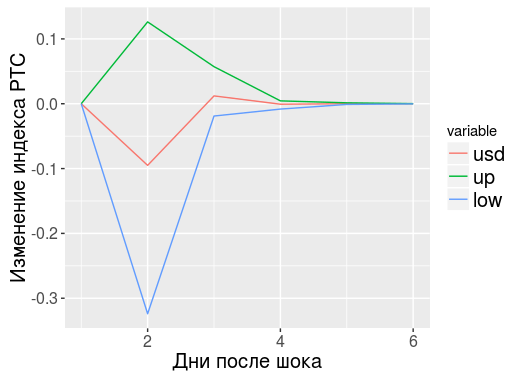
\includegraphics[width=1\linewidth]{Rplot_USD}}
\end{minipage}
\hfill
\begin{minipage}[H]{0.49\linewidth}
\center{\footnotesize{Индекс РТС} \\ 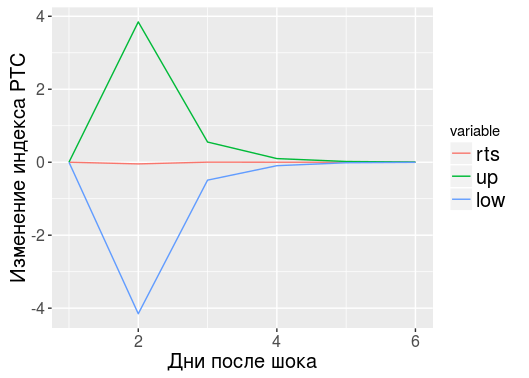
\includegraphics[width=1\linewidth]{Rplot_RTS}}
\end{minipage}
\vfill
\begin{minipage}[H]{0.49\linewidth}
\center{\footnotesize{Однодневная ставка МИАКР} \\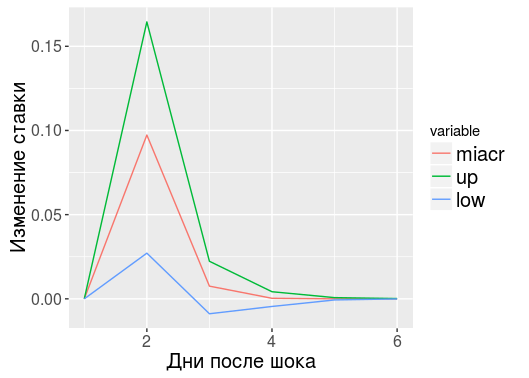
\includegraphics[width=1\linewidth]{Rplot_MIACR}} 
\end{minipage}
\caption{Функции импульсного отклика валютного курса, индекса РТС и ставки МИАКР на заявления Банка России}
\label{otkl_1}
\end{figure}

При словесной интервенции Банка России происходит прыжок однодневной ставки МИАКР в течение следующего дня после заявления. В течение четырёх дней ставка МИАКР возвращается к своему прежнему уровню. Вторая спецификация подтверждает выводы, полученные при первой спецификации модели. Импульсные отклики валютного курса и индекса РТС на словесные интервенции Банка России оказываются снова незначимыми.

\newpage

%%% Оформляем Заключение и список литературы также как Оглавление и Введение

\titleformat{\chapter} 
    {\normalfont\bfseries\large}
    {\noindent}{0em}{\centering\normalfont\bfseries}  


\chapter*{Заключение}
\addcontentsline{toc}{chapter}{Заключение}

Начиная с 2014 г. Банк России, в связи с переходом к режиму инфляционного таргетирования, начал иначе перестраивать свою информационную политику, повышая уровень предсказуемости и прозрачности. Управление ожиданиями постепенно налаживается, однако в Центробанке отмечают, что уровень репутации, необходимый для эффективного использования информационного канала, ещё не достигнут. 

В данной работе были рассмотрены различные методы анализа влияния словесных интервенций на динамику различных макроэкономических переменных. С их помощью был проведён анализ информационной политики Банка России.  

\nocite{*} 

\newpage

% Если хотим поменять название:
%\renewcommand{\refname}{Чтиво}  % По умолчанию "Список литературы" (article)
\renewcommand{\bibname}{Список литературы}  % По умолчанию "Литература" (book и report)

\printbibliography


%%%%%%%%%%%%%%%%%%%% Приложения %%%%%%%%%%%%%%%%%%%%

\newpage

\appendix
\renewcommand{\thechapter}{\Asbuk{chapter}}

%tocloft
\addtocontents{toc}{
\protect\renewcommand
\protect\cftchappresnum{Приложение~}
\protect\renewcommand
\protect\cftchapnumwidth{8.6 em}
}

%titlesec
\titleformat{\chapter}
 {\normalfont\bfseries\large}{\chaptertitlename~\thechapter.}{1 em}{\normalfont}

\titleformat{\section}{\bfseries}{\thesection}{1em}{}


\chapter[Программа~~  для~~ поиска~~ и~~ выгрузки~~   статей, касающихся Банка России из архива газеты Ведомости]{Программа для поиска и выгрузки статей, касающихся Банка Росии из архива газеты Ведомости (Python)}\label{app-a}

\begin{minted}[breaklines]{python}
def DaysOfYear(year):
    def Days(month):
        return([i for i in range(1,monthlength(month,2015)+1)])
    s = []
    for i in range(0,12):
        s.append(Days(i))
    return(s)
    
cd "C:\Users\zero\Desktop\mydata"

lll = DaysOfYear(2015)[0]
for number in lll:
    pickle.dump(getCBList(2015,1,number), 
    open(str(number)+'.txt', "wb" )) 
\end{minted}

Остальные месяцы выгружаются аналогичным образом. Теперь необходимо каждую из новостей, имеющих отношение к ЦБ дать оценку. Какой именно характер имеет словесная интервенция, отраженная в данной новости. Если она ведет к ужесточению политики, будем присваивать 1, если к смягчению, то -1. В итоге на выходе будем получать матрицу, каждая строка которой имеет вид [дата, смягчение или ужесточение].

\newpage
Выпускная квалификационная работа выполнена мной совершенно самостоятельно. Все использованные в работе материалы и концепции из опубликованной научной литературы и других источников имеют ссылки на них.

\vspace{2ex}

\noindent Объем работы  \rule{3em}{0.5pt} листа(ов).

\vspace{2ex}

\noindent Объем приложений \rule{3em}{0.5pt} листа(ов).

\vspace{4ex}

\noindent <<\rule{2em}{0.5pt}>> \rule{5em}{0.5pt} 201\rule{1em}{0.5pt} г. 

\vspace{4ex}

\noindent \rule{10em}{0.5pt} Ульянкин Филипп Валерьевич


\end{document}
